\chapter{Building Blocks for AI Agents}

\section{Board Evaluation}

When implementing an AI agent for games, especially strategy-based ones like Sagrada, the ability to evaluate the 
game board accurately is paramount. This evaluation serves as the foundation upon which the agent makes its decisions, 
determining the quality of its moves. By evaluating the board, the AI agent can 
prepare for future developments and plan its moves accordingly. It can identify key objectives, assess potential risks, 
and devise multi-step strategies to achieve its goals.  Evaluating the board efficiently is crucial for ensuring that 
the AI agent can process information and make decisions under a given time limit. 

\subsection{Board Evaluation in Sagrada} \label{subsec:Board_Evaluation_In_Sagrada}

Evaluating players' boards is one of the functionalities of the model component. The EvalState class is responsible for evaluating
the state of a given player including a board evaluation and the points for the unused favor tokens. Each EvalState object contains
the following components:
\begin{itemize}
    \item The penalty points received for the empty fields
    \item The number of Private Objective Card points received by the player
    \item A vector of PuocPatternState objects each representing the state of a concrete Public Objective Card
    \item The final score of the player that represents the number of points that the player would have if the game had ended before the evaluation
\end{itemize}


\subsubsection{PuocPatternState}
PuocPatternState objects represent the state of a board from the perspective of a given Public Objective Card. These objects
are constructed by the Public Objective Cards during the board evaluation. They contain both rules-based information 
(currently earned points) and heuristic-based information (the heuristic state).

The heuristic-based pattern evaluation is divided into completable and uncompletable patterns. The uncompletable
patterns are simply counted but for completable patterns, the number of dice that are missing to complete
the given pattern is remembered as well. This makes the evaluation of given patterns stronger because given agents can reward
placing dice that bring closer patterns to completion. 

The performance of an evaluation function is critical for agents using algorithms such as minimax, particularly in complex games 
such as Sagrada, where the branching factor is high. Certainly, there's often a trade-off between the accuracy and efficiency of an evaluation function. 
One of the inaccuracies occurs when evaluating Public Objective Cards that contain either a row or a column matching for unique dice colors or shades.
The reason behind this behavior is that each row/column is evaluated independently. However, the neighboring rows/columns have an impact on each other.

I will demonstrate this phenomenon in an example. Suppose that one of the Public Objective Cards is the Row Shade Variety. This means that the player is trying
to place dice so that each row will contain dice with unique shades. The following figure shows an example state:


\begin{figure}[H]
    \caption{ Incorrect evaluation board position example}
    \centerline{\mbox{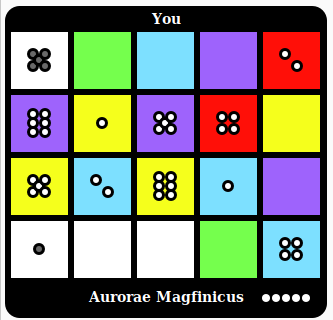
\includegraphics[width=100mm]{img/IncorrectBoardEvaluationExample.png}}}
    \label{fig:example}
\end{figure}


Notice that the second row could be completed with a 2 or a 3, and the third row could be completed with a 3 or a 4. Since the first row
contains a red die with the value of 2 at the rightmost column, a die having a value of 2 cannot be placed to the neighboring fields so the only 
value left for completing the second row is 3. The same principle applies to the third row and the blue 4 die in the fourth row. This means that 
both rows can be completed only with a 3 which is not possible at the same time because of the rules of the game. However, the board evaluation processes the rows
independently so it will report that both of these rows can be finished at the same time. The reason for not implementing it perfectly is connected
to performance. This phenomenon occurs rarely and avoiding it would require looking for a concrete placing of dice to each empty field. I decided 
that implementing this feature would not be worth the performance overhead.


\section{Heuristic Filter} \label{sec:Heuristic_filter}

Heuristic filters play a crucial role in AI algorithms, particularly in scenarios where exhaustive search or perfect evaluation is impractical due to 
computational constraints. Heuristic filters help narrow down the search space by quickly discarding unpromising choices, allowing the AI algorithm to 
focus its computational resources on more promising alternatives. 

One common pitfall is inadvertently limiting future placement options by positioning dice in a way that conflicts with the game's color or shade restrictions. 
Recognizing this, a heuristic filter can be employed to identify and avoid such ``bad moves'', both in regular die-to-field placements and when using Tool Cards.
When considering potential moves for placing a die on the board, the heuristic filter evaluates each option to determine if it would place a die adjacent to a field 
that shares the same color or shade restriction as the placed die. If such a placement is found, it's flagged as undesirable and filtered out. 
By proactively avoiding these conflicting placements, the AI ensures that it maintains flexibility and maximizes its future placement opportunities.
Similarly, when using Tool Cards, the heuristic filter explores the potential outcomes of each action to identify any placements that would create conflicts with 
existing dice on the board.

The Heuristic Filter is implemented in \texttt{the HeuristicFilter.h header file} that is part of the AI code of the project. The main function is the 
\texttt{void filter\_moves(Game\&, const vector<Move*>\& allMoves, vector<Move*>\& bestMoves, vector<Move*>\& backupMoves)} that receives all the moves to be filtered
and separates them into the \texttt{bestMoves} and \texttt{the backupMoves containers} using the filtering policy defined above.
The ``backup moves'' are used when there are no ``good moves'' to work with.

This technique is called ``forward pruning'' in the popular AI textbook \cite{norvig2002modern} . They say that ``Forward pruning prunes moves that appear to be poor moves, 
but might possibly be good Forward pruning ones. Thus, the strategy saves computation time at the risk of making an error''.

The following figure illustrates the impact of the Heuristic filter presented by the two AI agents that use it:
\begin{figure}[H]
    \caption{The impact of the Heuristic filter on the branching factor of two different AI players}
    \centerline{\mbox{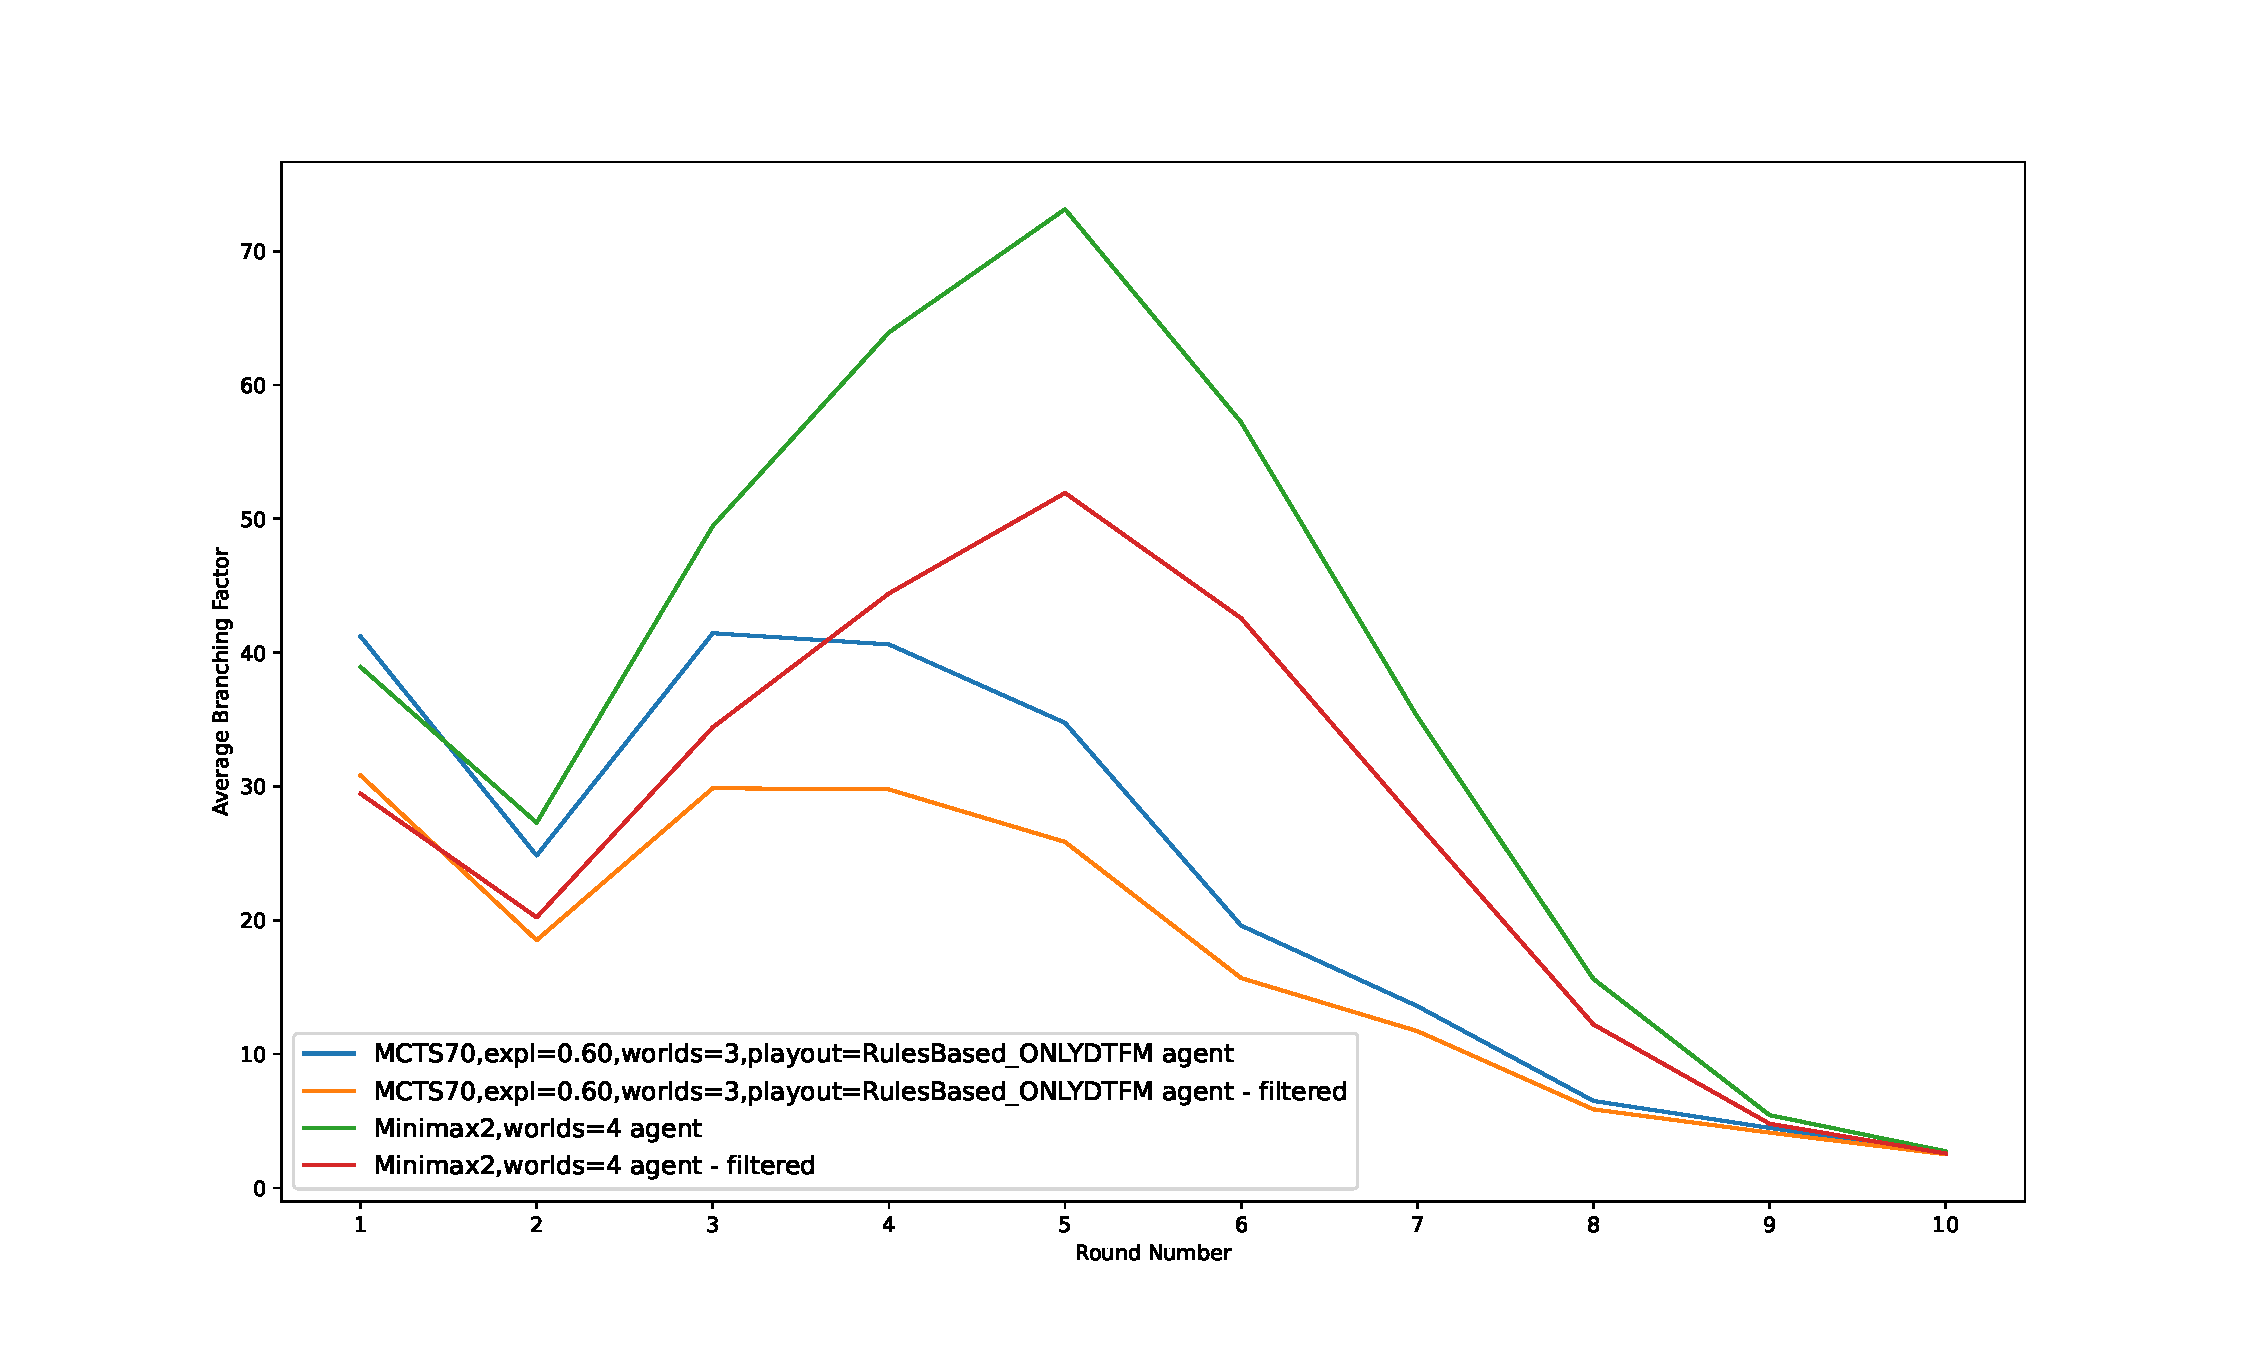
\includegraphics[width=180mm]{img/heuristic_filter.pdf}}}
    \label{fig:example}
\end{figure}

\section{Heuristic Sort} \label{sec:Heuristic_sort}

Heuristic sorting of moves plays a pivotal role in modern AI algorithms for board games, providing a strategic advantage by guiding the AI agent towards more promising moves. 
Furthermore, heuristic sorting facilitates the exploration of deeper and more complex game trees within a limited computational budget. In games with high branching factors, 
heuristic sorting allows AI agents to efficiently allocate their resources towards exploring the most promising branches of the game tree. Since the comparator is executed numerous times, 
its efficiency is critical to ensure the overall speed and responsiveness of the sorting algorithm.

In the previous section, I have already talked about filtering the least promising moves. This section provides a deeper understanding of how the remaining moves are sorted.
Due to the time limit, we cannot use any heuristic-based sorting technique that would be connected to the Public Objective Card patterns. There is one component in the scoring
structure that is easy to use as the basis of the sorting algorithm, namely the Private Objective Card's color.

The sorting algorithm decides between two moves according to the following criteria:
\begin{enumerate}
    \item If none of the moves is a die-placing move, a random move is prioritized
    \item If one of the moves is a die-placing move and the other one is not, the die-placing move is prioritized. 
    \item If one of the dice matches the color of the Private Objective Card and the other does not, the die matching the Private Objective Card color is prioritized.
    \item If one move places a die to a field that has a restriction and the other one does not, the one placed to a field with a restriction is prioritized.
    \item Finally, the die with the higher value is prioritized.
\end{enumerate}

The Heuristic Sort is implemented by \texttt{the comparator functor MoveHeuristicCMP} that is part of the AI code. It is designed to be used with \texttt{the std::sort algorithm} 
from the standard library as the comparator function.